\fancyhead[LE]{\fontsize{8.5pt}{10pt}\selectfont\textbf{\textsf{\thepage}}\quad \textbf{\textsf{CHƯƠNG 1}}\quad \textsf{Các hàm số và Mô hình}}
\fancyhead[RO]{\fontsize{8.5pt}{10pt}\selectfont\textsf{MỤC 1.1}\quad \textsf{Bốn cách biểu diễn một hàm số}\quad \textbf{\textsf{13}}}

\noindent
\begin{minipage}[t]{0.265\textwidth}
    \fontsize{8pt}{10pt}\selectfont
    \vspace*{240pt}
    \centering
    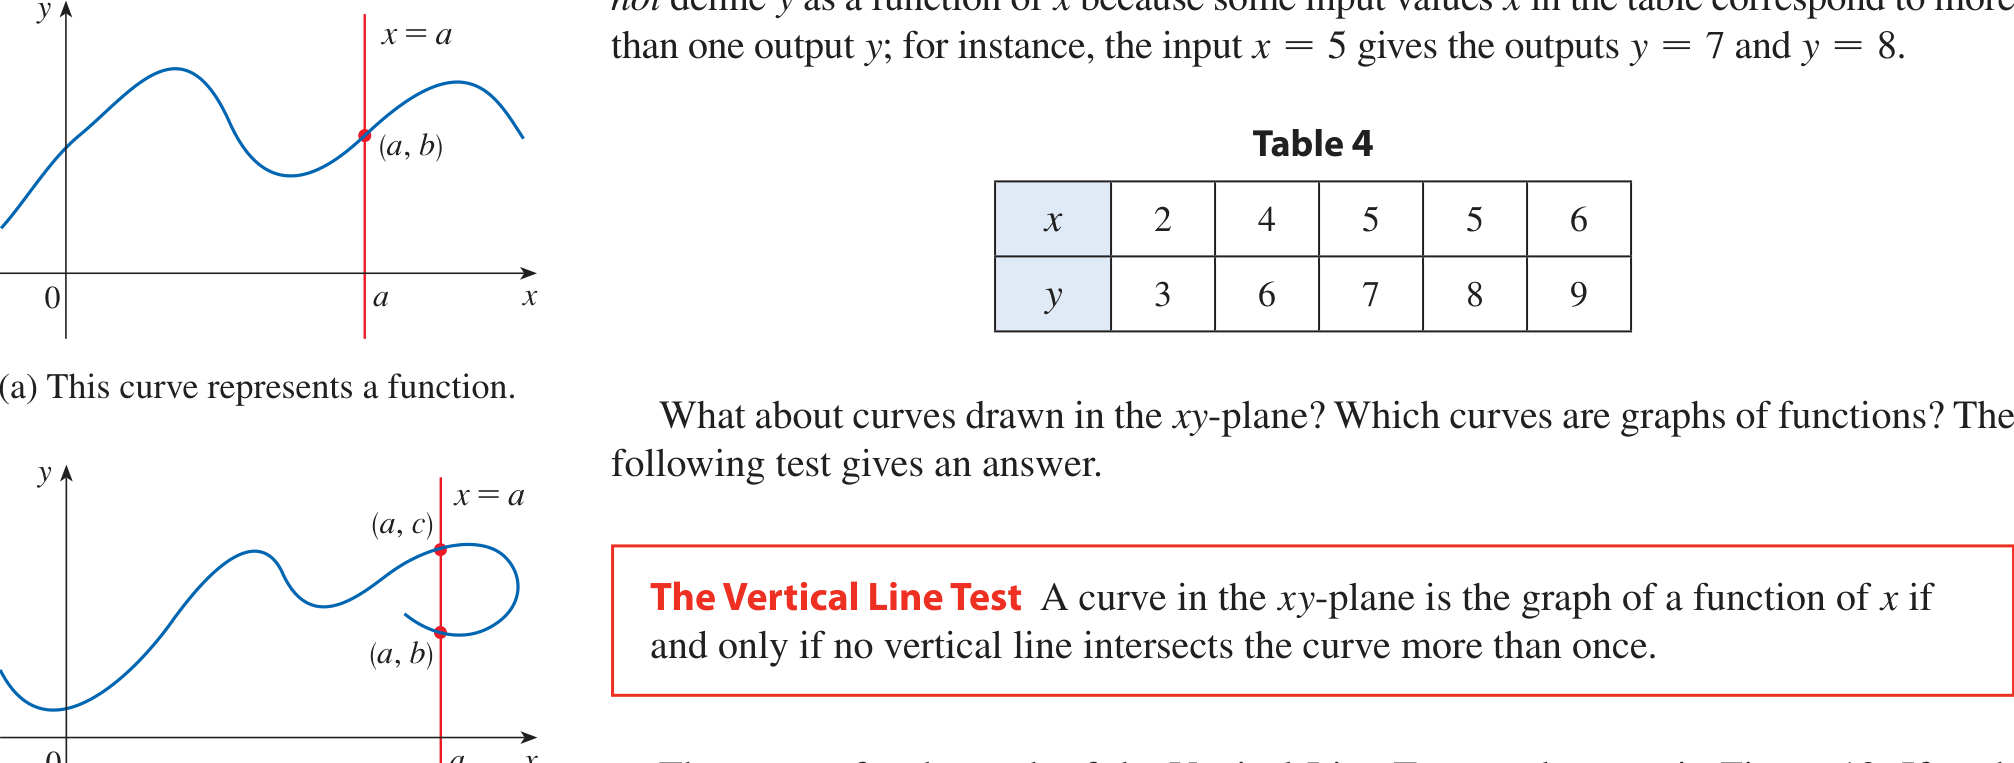
\includegraphics[width=0.92\linewidth]{images/p0048_fig13.png}
    \vspace{4pt}

    \raggedright
    \textbf{\textsf{HÌNH 13}}
\end{minipage}%
\hfill
\begin{minipage}[t]{0.708\textwidth}
    \fontsize{9.3pt}{13.2pt}\selectfont
    \noindent
    ...theo \textbf{quy ước tập xác định}: tập xác định của một hàm số là tập hợp tất cả các giá trị đầu vào sao cho công thức có nghĩa và cho ra kết quả là một số thực.

    \vspace{6pt}
    \noindent
    \textbf{\textsf{\color{stewartcyan}VÍ DỤ 6}}\quad Tìm tập xác định của mỗi hàm số sau:
    \vspace{3pt}

    \noindent
    (a) $f(x) = \sqrt{x + 2}$ \hfill (b) $g(x) = \dfrac{1}{x^2 - x}$

    \vspace{6pt}
    \noindent
    \textbf{\textsf{\color{stewartcyan}LỜI GIẢI}}
    
    \noindent
    (a) Vì căn bậc hai của một số âm không xác định (dưới dạng một số thực), nên tập xác định của $f$ bao gồm tất cả các giá trị của $x$ sao cho $x + 2 \geqslant 0$. Điều này tương đương với $x \geqslant -2$, do đó tập xác định là khoảng $[-2, \infty)$.

    \vspace{3pt}
    \noindent
    (b) Vì
    \[
    g(x) = \frac{1}{x^2 - x} = \frac{1}{x(x - 1)}
    \]
    và phép chia cho $0$ không được phép, ta thấy rằng $g(x)$ không xác định khi $x = 0$ hoặc $x = 1$. Do đó tập xác định của $g$ là
    \[
    \{x \mid x \neq 0, x \neq 1\}
    \]
    tập hợp này cũng có thể được viết bằng ký hiệu khoảng là
    \[
    (-\infty, 0) \cup (0, 1) \cup (1, \infty) \tag*{\color{stewartcyan}$\blacksquare$}
    \]

    \vspace{6pt}
    \noindent
    {\color{stewartcyan}\rule{1.2ex}{1.2ex}}\hspace{6pt}\textbf{\textsf{\large Những quy tắc nào xác định một hàm số?}}
    \vspace{4pt}

    \noindent
    Không phải mọi phương trình đều xác định một hàm số. Phương trình $y = x^2$ xác định $y$ là một hàm số của $x$ vì phương trình xác định duy nhất một giá trị của $y$ ứng với mỗi giá trị của $x$. Tuy nhiên, phương trình $y^2 = x$ \emph{không} xác định $y$ là một hàm số của $x$ bởi vì một số giá trị đầu vào $x$ tương ứng với nhiều hơn một giá trị đầu ra $y$; chẳng hạn, với giá trị đầu vào $x = 4$, phương trình cho hai giá trị đầu ra là $y = 2$ và $y = -2$.

    Tương tự, không phải mọi bảng giá trị đều xác định một hàm số. Bảng 3 đã xác định $C$ là một hàm số của $w$---mỗi khối lượng kiện hàng $w$ tương ứng với duy nhất một mức cước phí gửi thư. Mặt khác, Bảng 4 \emph{không} xác định $y$ là một hàm số của $x$ vì một số giá trị đầu vào $x$ trong bảng tương ứng với nhiều hơn một giá trị đầu ra $y$; chẳng hạn, giá trị đầu vào $x = 5$ cho hai giá trị đầu ra là $y = 7$ và $y = 8$.

    \begin{center}
        \textbf{\textsf{Bảng 4}}\\[4pt]
        \renewcommand{\arraystretch}{1.25}
        \begin{tabular}{|c|c|c|c|c|c|}
            \hline
            \rowcolor{stewartcyan!15} $x$ & 2 & 4 & 5 & 5 & 6 \\
            \hline
            \rowcolor{stewartcyan!15} $y$ & 3 & 6 & 7 & 8 & 9 \\
            \hline
        \end{tabular}
    \end{center}

    Còn các đường cong được vẽ trong mặt phẳng $xy$ thì sao? Những đường cong nào là đồ thị của hàm số? Phép thử sau đây sẽ cho ta câu trả lời.

    \vspace{4pt}
    \begin{definitionbox}
        \textbf{\textsf{\color{stewartred}Phép thử đường thẳng đứng}}\quad Một đường cong trong mặt phẳng $xy$ là đồ thị của một hàm số của $x$ khi và chỉ khi không có đường thẳng đứng nào cắt đường cong đó nhiều hơn một lần.
    \end{definitionbox}
    \vspace{4pt}

    Lý do cho tính đúng đắn của Phép thử đường thẳng đứng có thể được thấy ở Hình 13. Nếu mỗi đường thẳng đứng $x = a$ chỉ cắt đường cong đúng một lần, tại $(a, b)$, thì chỉ có duy nhất một giá trị hàm được xác định bởi $f(a) = b$. Nhưng nếu một đường thẳng $x = a$ cắt đường cong hai lần, tại $(a, b)$ và $(a, c)$, thì đường cong đó không thể biểu diễn một hàm số vì một hàm số không thể gán hai giá trị khác nhau cho cùng một giá trị $a$.
\end{minipage}